\section{Design considerations}
\label{section:inflex:design}

In chapter \ref{chapter:preflex}, one of the primary justifications for network assisted resource pooling was that existing solutions, such as \ac{MPTCP}, were not suitable for most flows. 
This assumption was founded on the fact that most flows were too short to make effective use of available bandwidth without prior knowledge of path quality.
The analysis in chapter \ref{chapter:rate} paints an even starker picture than was originally assumed: significant portions of traffic are limited and as such not inclined to make efficient use of capacity even if it were available.
With over half of all \ac{TCP} traffic constrained by factors other than loss, the allure of \ac{MPTCP} as a means of making use of all available end-to-end capacity between endpoints seems circumscribed to a small set of high-throughput transfers.

This suggests that the flexibility and robustness provided by resource pooling may be a more compelling feature than efficiency alone.
Despite being broadly designed for robustness, the current Internet architecture remains remarkably vulnerable to failures.
Managing faults still poses a significant operational challenge, in part because faults can occur at every layer of the networking stack, and can affect any element along a network path. 
\ac{PREFLEX} was designed with efficiency in mind, addressing resilience in passing.
In particular, \ac{PREFLEX} expects sufficient host feedback in order to adjust path weights.
This proves adequate for when many flows experience the same outage, but may fail to detect faults which affect isolated flows.
This chapter instead formulates a resource pooling architecture by first dealing with the single case -- addressing when a transport protocol detects failure -- and then extrapolating to the domain level, providing efficient traffic management.

\subsection{Latency}

While efficiency has become a less pressing concern for most traffic, latency has become increasingly valued, particularly as providers attempt to ensure responsive, interactive services.
This trend manifests itself in two manners within the \ac{MAWI} dataset.
Firstly, chapter \ref{chapter:malawi} detailed how significant volumes of traffic have been progressively shifted from transit to local peering links.
Given propagation delay is a critical component of end-to-end delay, putting content closer to end-users is an extremely effective method of cutting latency, and has assisted content distribution networks in becoming a key stakeholder within the Internet.
Secondly, flow rates for shorter transfers are increasing at a faster rate than for large flows, as displayed in figure \ref{fig:flowrate}.
Developments such as the increase of the initial window size \cite{Dukkipati:2010p160}, \ac{TCP} Fast Open \cite{Radhakrishnan:2011:TFO:2079296.2079317} coupled with higher socket limits and windowscale negotiation highlighted in chapter \ref{chapter:rate} have all benefited shorter flows disproportionately.

The original design of \ac{PREFLEX} imposes a potentially significant burden on latency by requiring network intervention at each flowlet.
While such network processing is small, and will necessarily improve over time, in hindsight tying together path selection and flowlet start does not feel entirely justified.
Chapter \ref{chapter:rate} demonstrated that over 40\% of all traffic is regularly application paced, and so the prevalence of opportunities for balancing at the flowlet level is unquestionable.
However, imposing network intervention on each flowlet start is excessive for short, delay-sensitive traffic, particularly since the benefit such small-grained balancing provides the network is negligible.
Requiring every \ac{PREFLEX} router to inspect packets on the basis of packet markings made by external entities was also a potential source of \acf{DoS}.
While such attacks are easily dismantled by rate limiting the number of \ac{FNE} packets received across network boundaries, at the very least this represents additional overhead for the operator, who must adequately configure and manage such a service.
As such, in considering an architecture for resilience, it would be beneficial to both instantiate network processing only when required and be robust to \ac{DoS} attacks by design.

\subsection{Deployment}

Ideally resilience could be implemented at the transport layer alone, for the same motives rate control is best left to end-hosts: ultimately, the host is best positioned to detect end-to-end path faults and can often react over shorter time scales than the network, which must concern itself with reconvergence.
This approach for path fail-over was a significant feature in \ac{SCTP} \cite{rfc4960}.
Unfortunately, deployment of \ac{SCTP} has been negligible in over a decade since standardization, in part because the pervasiveness of middleboxes has significantly affected the ability for new transport protocols to be deployed.
More recently \ac{MPTCP} has been proposed addressing many of the same concerns as \ac{SCTP} whilst maintaining the same wire format as \ac{TCP}, thereby ensuring middlebox compatibility.
Despite this, widespread deployment is far from guaranteed, and is largely tied to the rate of \ac{OS} adoption as evidenced in chapter \ref{chapter:rate}.

\begin{figure}[t]
    \centering
    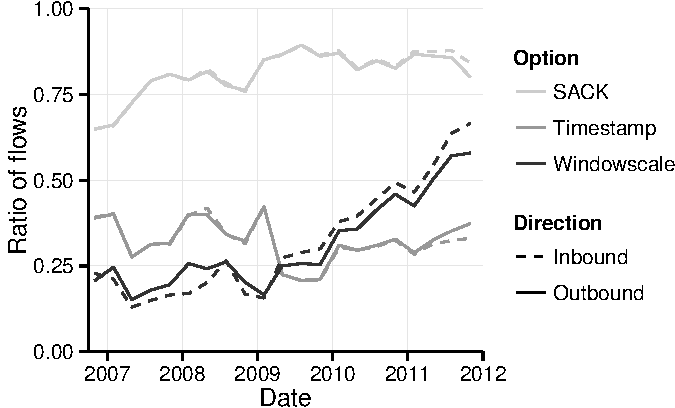
\includegraphics[width=4.0in]{figures/inflex/options}
    \caption{\acs{TCP} option usage.\label{fig:wscale}}
    \hfill
\end{figure}

As a reference point, figure \ref{fig:wscale} tracks the use of three \ac{TCP} options by overall volume in flows across both directions in the \ac{MAWI} dataset.
While \ac{SACK} is successfully negotiated for most connections, the deployment of the timestamp and windowscale options has lagged.
The former primarily assists in providing more accurate \ac{RTT} estimates and is therefore largely auxiliary.
The latter however is critical for performance: without windowscale negotiation, a sender's congestion window cannot exceed 65KB.
Despite offering a clear benefit to both endpoints, being simple to implement and incurring a low overhead, windowscale deployment has only recently picked up momentum, two decades since standardization.
Expecting substantial deployment of a more complex and costly extension such as \ac{MPTCP} over the near future is likely optimistic.
Critically, transport extensions require receiver adoption and are therefore subject to the willingness and ability of users to upgrade their OS.

This shortcoming affects \ac{PREFLEX} in equal measure.
The original assumptions for deployment in chapter \ref{chapter:preflex} were consistent with an Internet where traffic was mostly exchanged between peers.
Currently however, the asymmetry between the software which runs on either endpoint has never been greater, in large part due to the proliferation of mobile devices.
The barrier to deployment has been raised further: receiver side deployment of even modest \ac{TCP} extensions can be protracted, even when incentives are aligned.
Any proposed modification must find its way upstream to the code base of different \acp{OS} and be verified to perform adequately over a greater variety of constraints than in the desktop computing era.
Rather than proposing a path for incremental deployment, this chapter focuses instead on how to obtain similar benefits immediately -- modifying sender side hosts only. 

\subsection{Multipath routing}

A host, however, cannot directly affect routing without changing destination address, which would break legacy \ac{TCP} receiver side implementations. Additional extensions are required on the sender side network to enable multipath forwarding.
Conventional wisdom suggests that maintaining parallel routing planes requires a proportional increase in table size \cite{NingWang:2008p145}, which itself can be subject to exponential growth.
In practice however, this state can be significantly reduced by forsaking coverage for a small proportion of traffic.
Rather than reflect the entirety of its potential path diversity for all traffic, an edge provider can instead provide additional routing planes for only a subset of popular prefixes.

\begin{figure}[t]
    \begin{subfigure}[b]{0.5\linewidth}
        \centering
        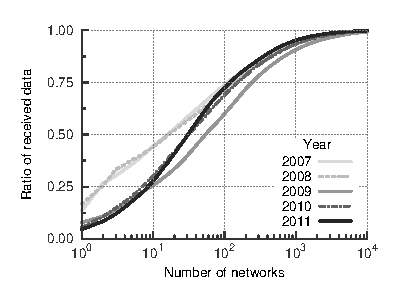
\includegraphics[width=0.95\linewidth]{figures/inflex/ecdf_network_dst_data_bytes_from_10000.eps}
        \caption{\label{prefix_in}}
    \end{subfigure}%
    \begin{subfigure}[b]{0.5\linewidth}
        \centering
        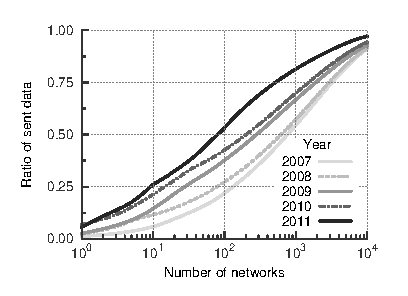
\includegraphics[width=0.95\linewidth]{figures/inflex/ecdf_network_dst_data_bytes_to_10000.eps}
        \caption{\label{prefix_out}}
    \end{subfigure}%
    \caption[\acs{CDF} of traffic by announced network prefix.]{\acs{CDF} of traffic by announced network prefix for (\subref{prefix_in}) inbound and (\subref{prefix_out}) outbound traffic.\label{fig:prefix}}
    \hfill
\end{figure}

The extent to which such a gain is possible for the \ac{MAWI} dataset is quantified in figure \ref{fig:prefix}, which displays the cumulative distribution function of outbound traffic across network prefixes announced by \ac{BGP} neighbours.
Over five years, traffic to approximately 340,000 unique prefixes was observed.
Invariably however, an increasing amount is sent to a small group of prefixes -- by 2011, over 50\% of traffic went to the top 100 prefixes alone.
As detailed in chapter \ref{chapter:malawi}, this reflects ongoing structural changes in the Internet architecture as content providers interconnect directly edge, \emph{eyeball} networks, and content becomes increasingly consolidated across a set of large content providers and national and regional ISPs.

\ac{PREFLEX} hinged on the fact that multipath routing state could be maintained and managed in a scalable manner, and these results demonstrate that multipath routing state can be significantly reduced by covering fewer destinations while still benefiting most traffic.
Within the \ac{MAWI} dataset virtually all inbound and outbound traffic could be mapped to 10,000 unique network prefixes. 
Existing tools such as RouteFlow \cite{Rothenberg:2012:RRC:2342441.2342445} are already capable of overlaying routing on commodity switches, but the incurred overhead can still be a concern for production networks.
Rather than address the scalability challenges inherent to multipath routing directly, these results suggest that a tangible deployment path lies instead in reducing the scope over which it is applied.

